\documentclass[12pt, twoside]{article}
\usepackage[a4paper, margin=0.9in]{geometry}
\usepackage{polski}
\usepackage[utf8]{inputenc}
\usepackage{graphicx}
\usepackage{xcolor,listings}
\usepackage{float}
\usepackage{rotating}
\usepackage{fancyhdr}
\usepackage{array}
\usepackage{amsmath}
\newcolumntype{M}{>{\centering\let\newline\\\arraybackslash\hspace{0pt}}m{2.5cm}}
\fancyhf{} % clear all header and footers
\renewcommand{\headrulewidth}{0pt} % remove the header rule
\fancyfoot[LE,RO]{\thepage} % Left side on Even pages; Right side on Odd pages
\pagestyle{fancy}
\fancypagestyle{plain}{%
	\fancyhf{}%
	\renewcommand{\headrulewidth}{0pt}%
	\fancyhf[lef,rof]{\thepage}%
}

\usepackage{hyperref}
\hypersetup{
	colorlinks,
	citecolor=black,
	filecolor=black,
	linkcolor=black,
	urlcolor=black
}

\begin{document}

\title{\vspace{50mm}Problem ośmiu hetmanów \\
	\large Sztuczna Inteligencja - Projekt	
}

\author{Dawid Paluch}
\date{\today}
\maketitle

\begin{center}
	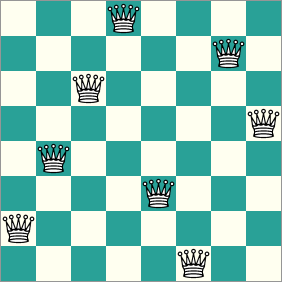
\includegraphics[keepaspectratio=true, scale=0.6]{8queens.png}
\end{center}
\thispagestyle{empty}
\clearpage
\setcounter{page}{1}

\clearpage
\tableofcontents
\clearpage

\setcounter{page}{3}
\section{Wprowadzenie}

\subsection{Problem ośmiu hetmanów}
W jaki sposób ustawić osiem hetmanów na szachownicy 8x8 by wzajemnie się nie atakowały? Ile jest możliwych ustawień?

\subsection{Historia problemu}
Problem ośmiu hetmanów został po raz pierwszy sformułowany w 1848 roku przez mistrza szachowego Maksa Bezzela (1824-1871). Pierwsze rozwiązanie podał dwa lata później Franz Nauck. Również matematyk Carl Friedrich Gauss interesował się tym problemem. W roku 1992 wskazano na związki pomiędzy problemem ośmiu hetmanów a kwadratami magicznymi.

\subsection{Reprezentacja rozwiązań}
Rozwiązania problemu przedstawiamy za pomocą ośmiu cyfr odpowiadających za kolejne kolumny szachownicy. Każda z cyfr określa wiersz na którym ustawiony jest hetman. Przykładowe rozwiązanie przedstawia rys. \ref{fig:example}.

\begin{figure}[H]
	\centering
	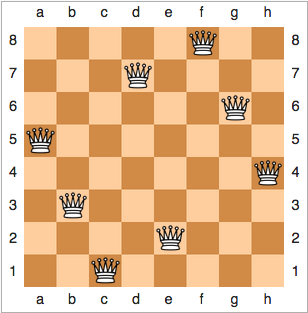
\includegraphics[keepaspectratio=true, scale=0.7]{example-53172864.png}
	\caption{Przykładowe rozwiązanie - 53172864}
	\label{fig:example}
\end{figure}

\clearpage
\section{Algorytm genetyczny}
\subsection{Opis algorytmu}
Problem ośmiu hetmanów możemy rozwiązać za pomocą algorytmu genetycznego. Populacją w naszym algorytmie będzie zbiór ustawień hetmanów. Każdy z osobników charakteryzuje się określonym dopasowaniem - im większe tym bliżej mu do prawidłowego rozwiązania.\\
Maksymalne dopasowanie dla problemu n-hetmanów określone jest wzorem:
\[ f_{max} = \dfrac{n(n - 1)}{2} \]
Co w przypadku problemu ośmiu hetmanów daje nam:
\[ f_{max} = \dfrac{8(8 - 1)}{2} = \dfrac{8 \cdot 7}{2} = 28 \]
Stopień dopasowania obliczymy odejmując liczbę atakujących się hetmanów(nazywaną też liczbą kolizji) od dopasowania maksymalnego:
\[ f = f_{max} - c\]
Osobniki z większym dopasowaniem będą miały większe prawdopodobieństwo reprodukcji, a co za tym idzie będą chętniej wybierane przez algorytm. Prawdopodobieństwo to dane jest wzorem:
\[ P(R) = \dfrac{f}{f_{max}}\]
Osobnik 42625782 będzie charakteryzował się dopasowaniem \( f = 24\) oraz prawdopodobieństwem reprodukcji \( P(R) = 0.857143\).
Po wybraniu dwóch osobników z możliwie najwyższym dopasowaniem następuje ich skrzyżowanie względem losowego punktu. 
Osobnik może zostać zmutowany z bardzo małym prawdopodobieństwiem np.
\[ P(C) = 0.03 \]
Mutacja osobnika polega na przesunięciu losowego hetmana na losowo wybrany wiersz.
\\[12pt]
Proces reprodukcji i ewentualnej mutacji będzie przebiegał aż do uzyskania w populacji osobnika z dopasowaniem maksymalnym, czyli z poprawnym rozwiązaniem problemu. W przypadku problemu ośmiu hetmanów otrzymamy ustawienie ośmiu hetmanów, które nie atakują się nawzajem.

\clearpage
\section{Podsumowanie}


\end{document}
